\chapter{Webscraping} \label{sec:Webscraping}
Web scraping is a method of automatically extracting content from web pages. The page from which the data is extracted is \hyperref[https://www.immonet.de/immobiliensuche/sel.do?suchart=2&fromarea=1.0&torooms=9999.0&city=87372&marketingtype=2&pageoffset=1&radius=0&parentcat=1&listsize=26&sortby=0&objecttype=1&fromrooms=1.0&fromprice=1.0&page=1]{}{}{}{immonet.de}\footnote{ It is important to use the correct URL, because the URL contains the filter settings and the information that the first page is displayed (Page-1). For example, a For loop can be used to access different pages. \hyperref[https://www.immonet.de/immobiliensuche/sel.do?suchart=2&fromarea=1.0&torooms=9999.0&city=87372&marketingtype=2&pageoffset=1&radius=0&parentcat=1&listsize=26&sortby=0&objecttype=1&fromrooms=1.0&fromprice=1.0&page=2]{}{}{}{https://www.immonet.de/immobiliensuche/sel.do?suchart=2\&fromarea=1.0\&torooms=9999.0\&city=87372\& marketingtype=2\&pageoffset=1\&radius=0\&parentcat=1\&listsize=26\&sortby=0\&objecttype=1\&fromrooms=1.0\& fromprice=1.0\&page=1}}. Some filter settings were used to exclude unfavorable data from the outset:

\begin{description}
	\item[Ort] Used as a variable during readout. For example Berlin\footnote{In the URL the code city=87372 is used for this purpose}.
	\item[Was] Exclusively apartments - no houses or land 
	\item[Preis] from  1 EUR -  some rental prices are only communicated 'on request'. With the filter these properties will be ignored.
	\item[FLäche] from  $1 \ m^2$ -  For the calculation of a price per square meter, the area is essential
	\item[Zimmer] 1 - 999 - In order to prevent possible problems with the readout from the outset
\end{description} 

The website immonet.de delivers 444 hits for Berlin at the time of writing this seminar paper. There is an ID for each property. With this unique ID, the concrete property can be called up in turn. This unique ID ultimately provides the URL of the apartment and can be determined as follows:

\begin{verbatim}
	page<-read_html("https://www.immonet.de/immobiliensuche/sel.do?suchart=2&
	fromarea=1.0&torooms=9999.0&city=87372&marketingtype=2&
	pageoffset=1&radius=0&parentcat=1&listsize=26&sortby=0&
	objecttype=1&fromrooms=1.0&fromprice=1.0&page=1")
	page %>%
	html_elements(".flex-grow-1.overflow-hidden.box-25 a")%>%
	html_attr("href")
\end{verbatim}

This results in 26 ID's for the first page.
\begin{verbatim}
	ids
	1  /angebot/47032733
	2  /angebot/49369370
	3  /angebot/49357545
	.
	.
	.
	24 /angebot/49187554
	25 /angebot/49178201
	26 /angebot/48180027
\end{verbatim}

The combination of the URL immonet.de and the first ID provides the URL immonet.de/angebot/47032733 to a specific property. The URL is used to get to the properties of the real estate. This procedure was carried out for 20 cities. This resulted in a total of 6520 data records on 23.12.2022. The verification of the correctness of the data revealed some problems that will be addressed in the rest of the paper.


\section{Problems of the data set}

After the data set was completely extracted, the data was checked for plausibility. In the process, some errors were noticed on the website. Before the check, a definition for the warm rent and the cold rent had to be created.

The warm rent refers to the rent including all ancillary costs and the heating costs. Also included are any costs for garage parking spaces. The cold rent, on the other hand, viewed from the perspective of an investor, represents the return on the property. Since ancillary costs and heating costs must be borne by the tenant, the cold rent is defined as rent without any other costs.

Inconsistencies were noticed when reviewing the data.

\subsection{Warm rent = cold rent}
Somewhat unusual is the fact that for some properties the warm rent corresponded to the cold rent. Upon closer inspection, it turned out that these were either furnished apartments or student or senior housing with assisted living. Flat rents are nothing unusual in this context. Basically, this is not an error of the data set, but a limitation of the readout process, since this information is only available as text and an additional analysis of the texts would have been necessary to extract this information. 

\begin{figure}[H]
	\centering
	
\includegraphics[width=0.7\linewidth]{img/49069527}
	\caption{Error: warm rent = cold rent}
	\label{fig:49069527}
\end{figure}

\subsection{Cold rent > Warm rent}

The cold rent was greater than the warm rent. Initially, the assumption was that the data had not been read out correctly. However, after closer examination, it could be determined that the operators of Immonet.de do not check the data for plausibility before publishing the advertisement. As can be seen in the figure \ref{fig: error kalt > warm} for example, the ID's 47122153 and 48642772 provide a larger cold rent than warm rent. This is obviously wrong, but a closer look shows that warm and cold rent were swapped here. In total, there were 5 records that were incorrect in this area. 4 records were corrected and one was removed. 

\begin{figure}[H]
	\begin{center}
		\begin{minipage}{0.4\textwidth}
			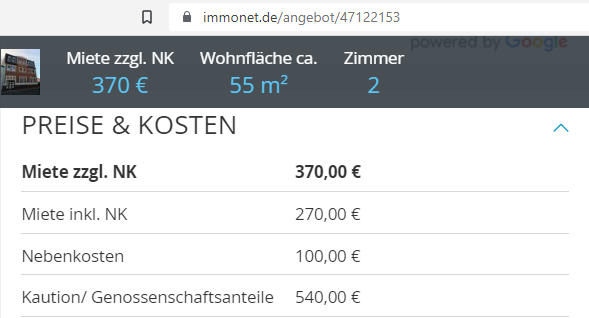
\includegraphics[width=0.7\linewidth]{img/47122153}
		\end{minipage}
		\begin{minipage}{0.4\textwidth}
			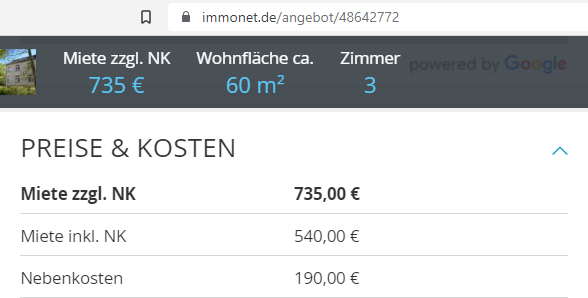
\includegraphics[width=0.7\linewidth]{img/48642772}
		\end{minipage}
	\end{center}
	\caption{Error: Cold rent > Warm rent }
	\label{fig: error kalt > warm}
\end{figure}

\subsection{Heating costs included in warm rent}
The page offers two fields to determine whether the heating costs are included in the warm rent or in the service charges or not. Quite obviously, there are problems of confusion here. The figure \ref{Error: Heizkosten in Warmmiete} shows that the difference between warm rent and cold rent is the same as the indicated heating costs. It can be assumed that in these cases the heating costs are included in the service charges instead of in the warm rent as indicated.
\begin{figure}[H]
	\begin{center}
		\begin{minipage}{0.4\textwidth}
			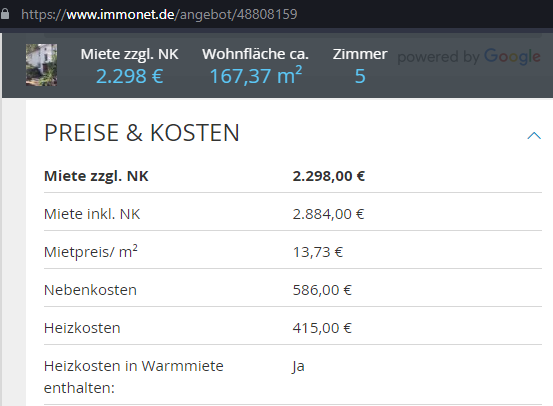
\includegraphics[width=0.7\linewidth]{img/48808159}
		\end{minipage}
		\begin{minipage}{0.4\textwidth}
			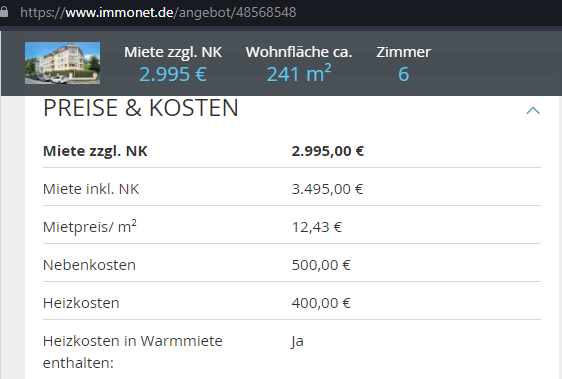
\includegraphics[width=0.7\linewidth]{img/48568548  }
		\end{minipage}
	\end{center}
	\caption{Error: Heating costs = ancillary costs?  }	
	\label{Error: Heizkosten in Warmmiete}
\end{figure}

In addition, there are problems with the query whether the heating costs are included in the service charges. The figure \ref{fig: Heikosten in NK} shows that the sum of cold rent and service charges does not correspond to the warm rent. It is likely that the figure indicates that the heating costs are included in the warm rent.

\begin{figure}[H]
	\centering
	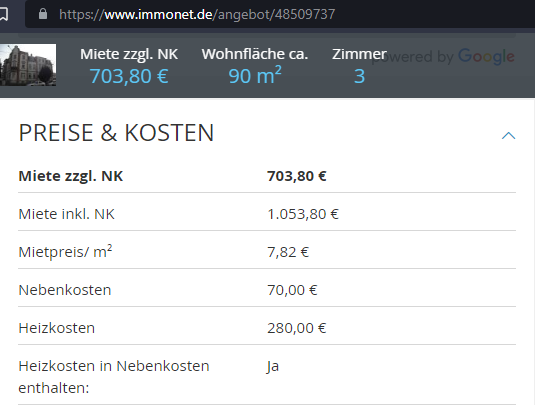
\includegraphics[width=0.7\linewidth]{img/48509737}
	\caption{Error:  Heating costs in ancillary costs}
	\label{fig: Heikosten in NK}
\end{figure}


\subsection{Garage}

An additional problem is the indication of the garage. There are cases when garage parking spaces belong to a property and the price for this parking space is specified. In some cases the price of the garage parking space is included in the cold rent, in other cases it is not. There are also cases where the price for the garage parking space is included in the warm rent, in other cases it is not. These data have been corrected, if it was possible, to ensure the correctness of the data. 



\subsection{Interim summary}

The initial analysis of the data highlighted a flawed data set. Some differences between cold and warm rent could not be clearly determined. Often, the erroneous difference was only a few euros. These errors were accepted because they may not have been significant enough to affect the analysis. Some data were still wrong despite all assumptions, which is illustrated by the figure \ref{Error: allgemeine Fehler}.  However, this type of error can be corrected by the subsequent outlier analysis. It should be noted that the poor quality of the data did not result from the readout, but that the operators of Immonet.de did not have the data checked by a program before publication. Only a few additional queries would be required to significantly improve the data quality. The fact that the data quality is poor could cause problems in the modeling. The following is an analysis of the data set first.

\begin{figure}[H]
	\begin{center}
		\begin{minipage}{0.4\textwidth}
			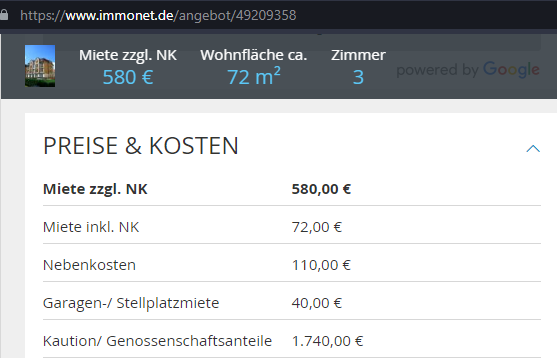
\includegraphics[width=0.7\linewidth]{img/49209358}
		\end{minipage}
		\begin{minipage}{0.4\textwidth}
			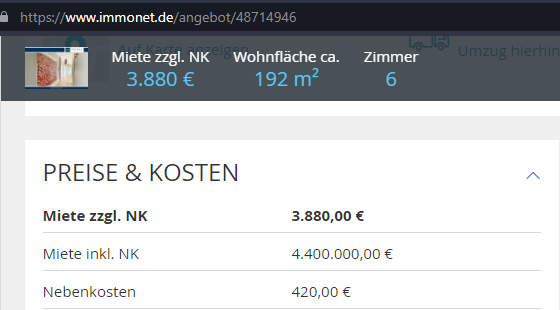
\includegraphics[width=0.7\linewidth]{img/48714946  }
		\end{minipage}
	\end{center}
	\caption{Error: Heating costs = ancillary costs? }
	\label{Error: allgemeine Fehler}
\end{figure}